\documentclass[class=article,crop=false]{standalone}
\usepackage{default}
\usepackage{booktabs}
\usepackage{adjustbox}
\usepackage{caption}

\begin{document}

Luego de bajar los datos fue necesario ajustar las unidades de las variables de interes. Los datos de presión se pasaron de [hPa] a [Pa], y la temperatura de [$^\circ$C] a [K]. También se transformó la razón de mezcla (en [g/Kg]) a la humedad especifica $q$ (adimensional).

\begin{enumerate}[a)]
    \item La temperatura virtual $T_v$ la calculamos para cada fila de datos usando la expresión
\begin{equation}
T_v = T(1+0.61 q) \label{Tv}
,\end{equation}
donde $T$ es la temperatura en Kelvin y $q$ la humedad específica. Por otro lado, la densidad $\rho$ fue obtenida a partir de la ecuación de estado, es decir
\begin{equation}
\rho = \frac{P}{R_d T_v},
\end{equation}
con $P$ la presión y $R_d = 287.04 \left[\frac{\text{J}}{\text{Kg}\,\text{K}}\right]$ 
\item \textbf{Para Z1} se consideraron la siguientes expresiones de la atmósfera standard.
\begin{equation}
T(z) = T_0 + mz \label{isaT}
\end{equation}
\begin{equation}
P(z) = P_0 \left(\frac{T(h)}{T_0}\right)^{-\dfrac{g}{m\,R_d}} \label{isaP}
\end{equation}
La ecuación \eqref{isaT} indica que la temperatura decrese de forma lineal con la altura, a una $m$. Además se asume que la temperatura en la superficie ($z=0$) es $T_0$. Por otro lado, \eqref{isaP} muestra como la presión depende de la temperatura y del gradiente de temperatura ($m$). Para relacionar ambas cantidades remplazamos \eqref{isaT} en \eqref{isaP}. Luego nos queda
\begin{align*}
    P &= P_0 \left(\frac{T_0 + mz}{T_0}\right)^{-\frac{g}{m\,R_d}} \\
    \left(\frac{P}{P_0}\right)^{-\frac{m\,R_d}{g}} &= \frac{T_0 + mz}{T_0} \\
    T_0\left(\frac{P}{P_0}\right)^{-\frac{m\,R_d}{g}} &= T_0 + mz \\
    T_0\left[\left(\frac{P}{P_0}\right)^{-\frac{m\,R_d}{g}} -1 \right] &= mz 
\end{align*}
Con esto obtenemos que la altura es
        \begin{equation}
            \text{Z1} = \frac{T_0}{m}\left[\left(\frac{P}{P_0}\right)^{-\frac{m\,R_d}{g}} -1 \right]  \label{Z1}
        \end{equation}
Consideraremos $T_0$ y $P_0$ como los valores de temperatura y presión del primer nivel (primera fila de datos), y $m =-6.5/1000$ (indicando que la temperatura disminuye en 6.5$^\circ$C cada 1000 metros) , $R_d = 287.04$ [J/Kg K], y $g= 9.78$ [m/s$^2$]. 
Entonces, usamos la ecuación \eqref{Z1} en cada fila de datos para obtener la altura Z1.

\textbf{Para Z2} se consideró la ecuación hipsométrica dada por
\begin{equation}
\text{Z2}_2 - \text{Z2}_1 = \frac{R_d \langle T \rangle }{g} \ln\left(\frac{P_1}{P_2}\right) 
\end{equation}
con $\langle T \rangle$ el promedio de las temperaturas virtuales en los puntos 1 y 2. Como esta ecuación nos proporciona el espesor entre dos puntos, se calculó el espesor entre cada par consecutivo de datos, y luego se hizo una suma acumulativa para registrar Z2. \\

A continuación presentamos las tablas con los datos.



	\captionsetup[table]{font=scriptsize}
	\begin{minipage}{0.49\linewidth}
	\captionof{table}{Radiosondeo del 15 de enero de 1997 (Verano)}
	\begin{adjustbox}{width=\linewidth}
	\import{.}{tbl1.tex}
	\end{adjustbox}
	\end{minipage}
	\hfill
	\begin{minipage}{0.49\linewidth}
	\captionof{table}{Radiosondeo del 15 de Agosto de 1997 (Invierno)}
	\begin{adjustbox}{width=\linewidth}
	\import{.}{tbl2.tex}
	\end{adjustbox}
	\end{minipage}

\item A continuación mostramos los perfiles de temperatura\\
    \begin{minipage}{0.49\linewidth}
        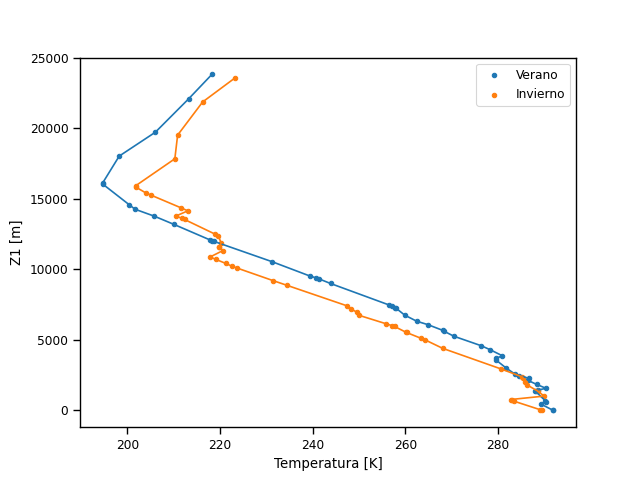
\includegraphics[width=1.1\linewidth]{Z1.png}
        \captionof{figure}{Temperatura en relación a la altura Z1}
    \end{minipage}
        \hfill
    \begin{minipage}{0.49\linewidth}
        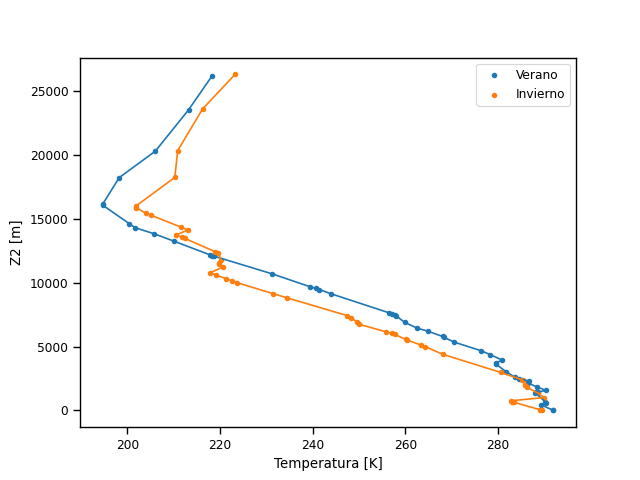
\includegraphics[width=1.1\linewidth]{Z2.png}
        \captionof{figure}{Temperatura en relación a la altura Z2}
    \end{minipage}

    Notamos como en ambas figuras, a baja altura ($z<10000$m) la temperatura es mayor para el registro de verano, aunque para el registro de invierno, los datos de mas baja altura presentan harta variación. \\
    De las tablas podemos notar que en el registro de verano hay mas humedad específica $q$. Esto podría deberse a que la estación de radiosondeos se encuentra en Antofagasta, cercano a la costa, donde las altas temperaturas provocan más vaporización del agua del mar. 


\end{enumerate}

\end{document}
